\subsection{Mikrocontroller} \label{sec:microcontrollerHardware}

Als Microcontroller wurde ein nRF52832 der Firma Nordic Semiconductors verwendet, welcher in Abbildung \ref{fig:nRF52832} ersichtlich ist. Seine hohe Performance ermöglicht es ein System aufzubauen, welches den Microcontroller als zentrale Schnittstelle beinhaltet. Der Microcontroller bildet gemäss der Abbildung \ref{fig:Teilsysteme} in Kapitel \ref{sec:gesamtkonzept} bereits beschrieben das Herzstück des Dōjōs. 

\begin{figure}[H]
	\begin{center}
		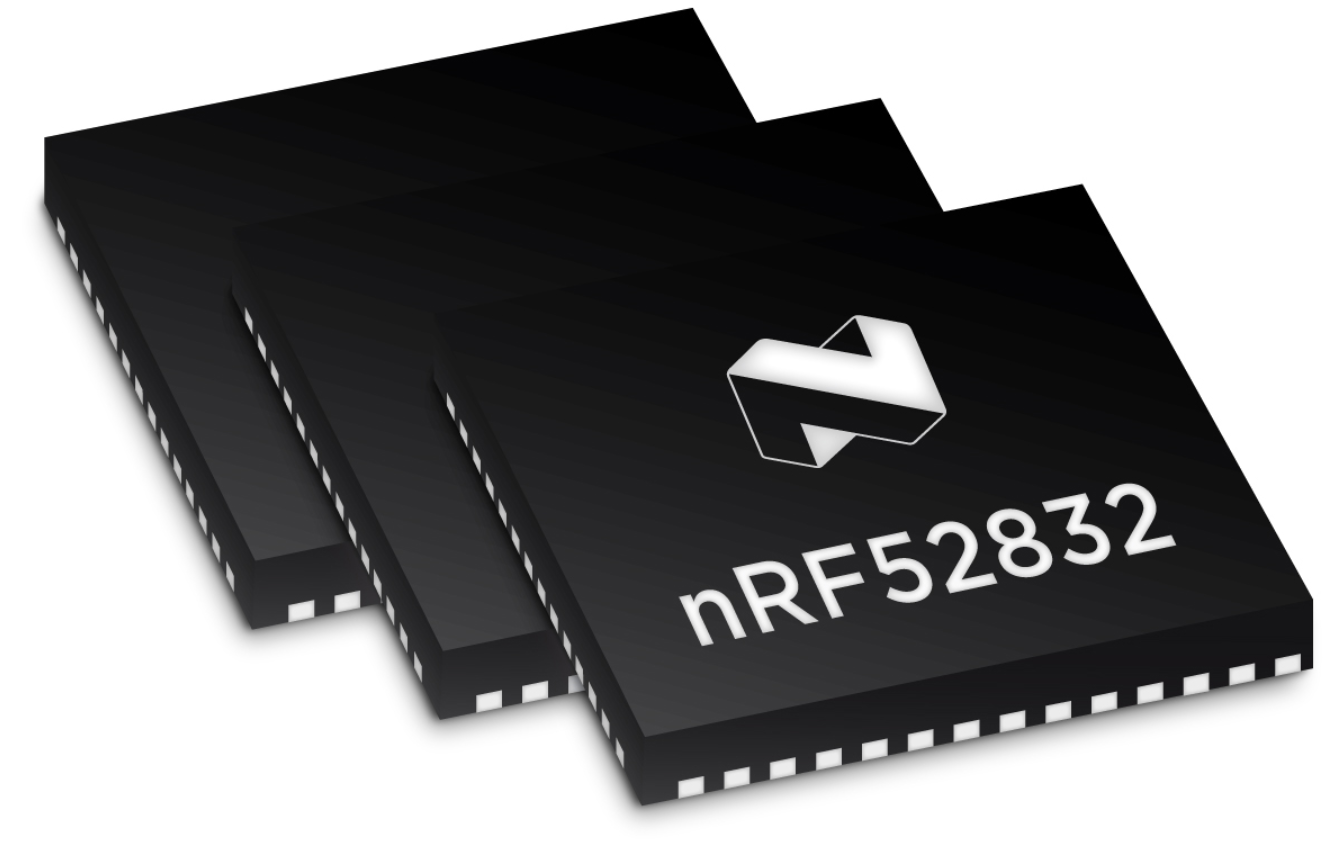
\includegraphics[width=60mm]{data/nRF52832.png}
		\caption[nRF52832 Microcontroller]{nRF52832 Microcontroller \cite{nRF52832}} %picture caption
		\label{fig:nRF52832}
	\end{center}
\end{figure}

Der nRF52832 weist eine Betriebsversorgungsspannung zwischen 1.7V und 3.6V mit einem Versorgungsstrom von 5.4mA auf. Diese niedrigen Werte ermöglichen somit einen dauerhaften Betrieb durch die integrierte Batterie. Die Speicherkapazität ist durch 512kB flash/64kB RAM Speicher gegeben. Für ein einfacheres Handling beim programmieren zu erreichen, wurden für die ersten Tests ein Development Kit (Abbildung \ref{fig:nRF52832-DK}) mit intergriertem nRF52832 verwendet.

\begin{figure}[H]
	\begin{center}
		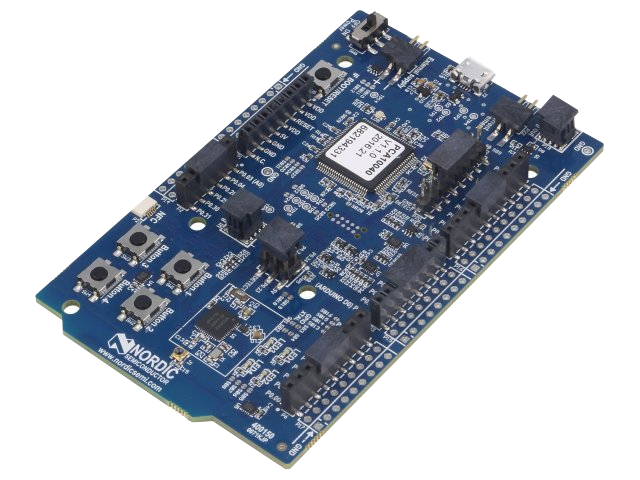
\includegraphics[width=100mm]{data/NRF52-DK.png}
		\caption[nRF52 Development Kit]{nRF52 Development Kit \cite{nRF52-DK}} %picture caption
		\label{fig:nRF52832-DK}
	\end{center}
\end{figure}
 Die Schlüsselmerkmale dieses Boards sind zum einen wie bereits beschrieben der integrierte Microcontroller, zum anderen aber auch eine integrierte Bluetooth Antenne. Das Kit unterstützt zudem proprietäre Bluetooth Smart, ANT und 2.4GHz Applikationen. Es ermöglicht aber auch den Einsatz von Drittanbieter Shields. Dies ermöglicht das Beschreiben und Lesen der SD-Karte zu testen.
